%%% PREAMBLE

\documentclass{article}
\usepackage{amsmath,amssymb,amsthm,fullpage,graphicx,subcaption}

% Use break between paragraphs instead of indentation
%\usepackage{parskip}

% Code highlighting
\usepackage[utf8]{inputenc}
\usepackage{listings, color}

% Default fixed font does not support bold face
\DeclareFixedFont{\ttb}{T1}{txtt}{bx}{n}{9} % for bold
\DeclareFixedFont{\ttm}{T1}{txtt}{m}{n}{9}  % for normal

% Custom colors
\usepackage{color}
\definecolor{deepblue}{rgb}{0,0,0.5}
\definecolor{deepred}{rgb}{0.6,0,0}
\definecolor{deepgreen}{rgb}{0,0.5,0}

% Python style for highlighting
\newcommand\pythonstyle{\lstset{
language=Python,
basicstyle=\ttm,
otherkeywords={self},             % Add keywords here
keywordstyle=\ttb\color{deepblue},
emph={MyClass,__init__},          % Custom highlighting
emphstyle=\ttb\color{deepred},    % Custom highlighting style
stringstyle=\color{deepgreen},
frame=tb,                         % Any extra options here
showstringspaces=false,           % 
commentstyle=\ttm\color{magenta}
}}

% Python environment
\lstnewenvironment{python}[1][]
{
\pythonstyle
\lstset{#1}
}
{}

% Python for external files
\newcommand\pythonex[2][]{{
\pythonstyle
\lstinputlisting[#1]{#2}}}

% Python for inline
\newcommand\pyln[1]{{\pythonstyle\lstinline!#1!}}

% Various math conveniences
\theoremstyle{definition}
\newtheorem*{prop}{Proposition}
\newtheorem*{obs}{Observation}
\newtheorem*{lemma}{Lemma}
\newtheorem*{disc}{Discussion}
\newtheorem*{qn}{Question}
\renewcommand{\bar}{\overline}
\newcommand{\nin}{\not\in}
\renewcommand{\>}{\rangle}
\newcommand{\<}{\langle}



%%% FILE INFO

% Header
%\usepackage{fancyhdr}
%\usepackage[margin=1in, headheight=50pt]{geometry}
%\pagestyle{fancy}
%\lhead{\textbf{CS21}}
%\chead{Final}
%\rhead{Aritra Biswas}
%\setlength{\headsep}{20pt}

% Title stuff
\title{\textbf{Set 3: Numerical methods for ODEs}}
\date{}
\author{Aritra Biswas}



%%% DOCUMENT

\begin{document}

\maketitle

\section{Implementation of explicit Euler Method}

We have:
\begin{align*}
F = m\frac{d^2 x}{dt^2} &= -kx \\
\frac{d^2 x}{dt^2} &= -\frac{k}{m} x
\end{align*}
Under our simplification that $\frac{k}{m}=1$:
\begin{align*}
\frac{d^2 x}{dt^2} &= -x
\end{align*}
We use the explicit Euler method to approximate a solution
to this ODE:
\begin{align*}
x(t+h) &\approx x(t) + h\frac{dx}{dt} \\
x_{i+1} &= x_i + hv_i. \\
v(t+h) &\approx v(t) + h\frac{dv}{dt} \\
v_{i+1} &= v_i - hx_i.
\end{align*}
\begin{minipage}{\textwidth}
\pythonex[firstline=4, lastline=25]{spring.py}
\end{minipage}

With initial conditions $x_0 = 0$, $v_0 = 5$, and a step
size $h=0.05$ with a stop time $s=50$, the above subroutine produces
the numerical solutions for $x(t)$ and $v(t)$ shown in figure \ref{fig:explicit}.

\begin{figure}
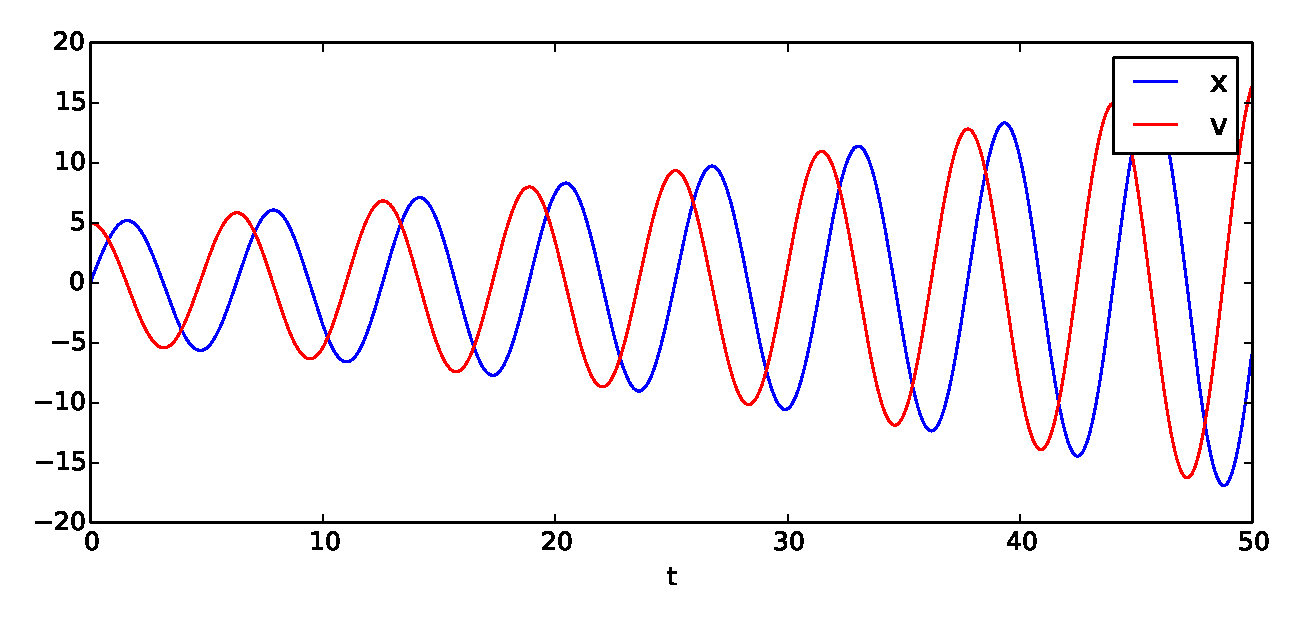
\includegraphics[width=\textwidth]{explicit.eps}
\caption{\label{fig:explicit}Numerical solutions for $x(t)$ and $v(t)$ as calculated
by the explicit Euler method.}
\end{figure}

\section{Comparison with analytic solution}

We show that a generic sinusoidal function is a solution
to the given ODE.
\begin{align*}
x &= A\sin t + B\cos t \\
v = \frac{dx}{dt} &= A\cos t - B\sin t \\
\frac{d^2 x}{dt^2} &= -A\sin t - B\cos t = -x
\end{align*}
Using our initial values $x=x_0$ and $v=v_0$ at $t=0$:
\begin{align*}
x_0 &= A\sin 0 + B\cos 0 \\
    &= B. \\
v_0 &= A\cos 0 - B\sin 0 \\
    &= A.
\end{align*}
Thus, the complete analytical solution is:
\begin{align*}
x &= v_0\sin t + x_0\cos t. \\
v &= v_0\cos t - x_0\sin t.
\end{align*}
Figure \ref{fig:explicit_error} shows the global trunctation error,
the difference between the
explicit Euler method used in section 1 and the analytic method derived
here. The error is computed in the \pyln{global_error} function:
\begin{minipage}{\textwidth}
\pythonex[firstline=70, lastline=97]{spring.py}
\end{minipage}

\begin{figure}
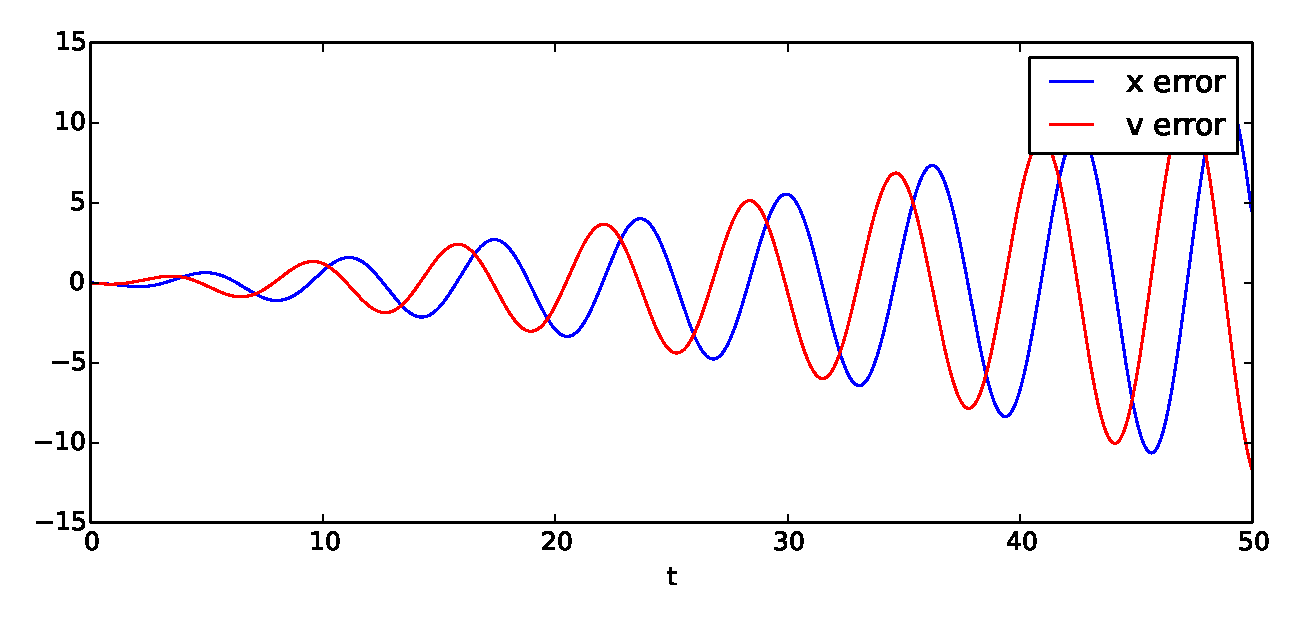
\includegraphics[width=\textwidth]{explicit_error.eps}
\caption{\label{fig:explicit_error}Truncation error:
difference between the analytic solution and the
solution calculated from the explicit Euler method.}
\end{figure}

\section{Relationship between truncation error and step size $h$}

We examine the effect of changing the step size $h$ on the truncation error
with the following subroutine \pyln{error_vs_h}, which plots the
maximum truncation error for various $h$ ranging from a given $h_0$ to
$\frac{h_0}{16}$.

\pythonex[firstline=99, lastline=123]{spring.py}

Figure \ref{fig:bigh} shows an exponential trend for various,
somewhat large $h$ ($h_0 = 0.1)$.
If we restrict the domain to small $h$, we expect to see a small portion of
this exponential curve, which will appear linear.
As expected, figure \ref{fig:smallh} shows a roughly linear trend
when $h$ is small ($h_0 = 0.01)$.

\begin{figure}
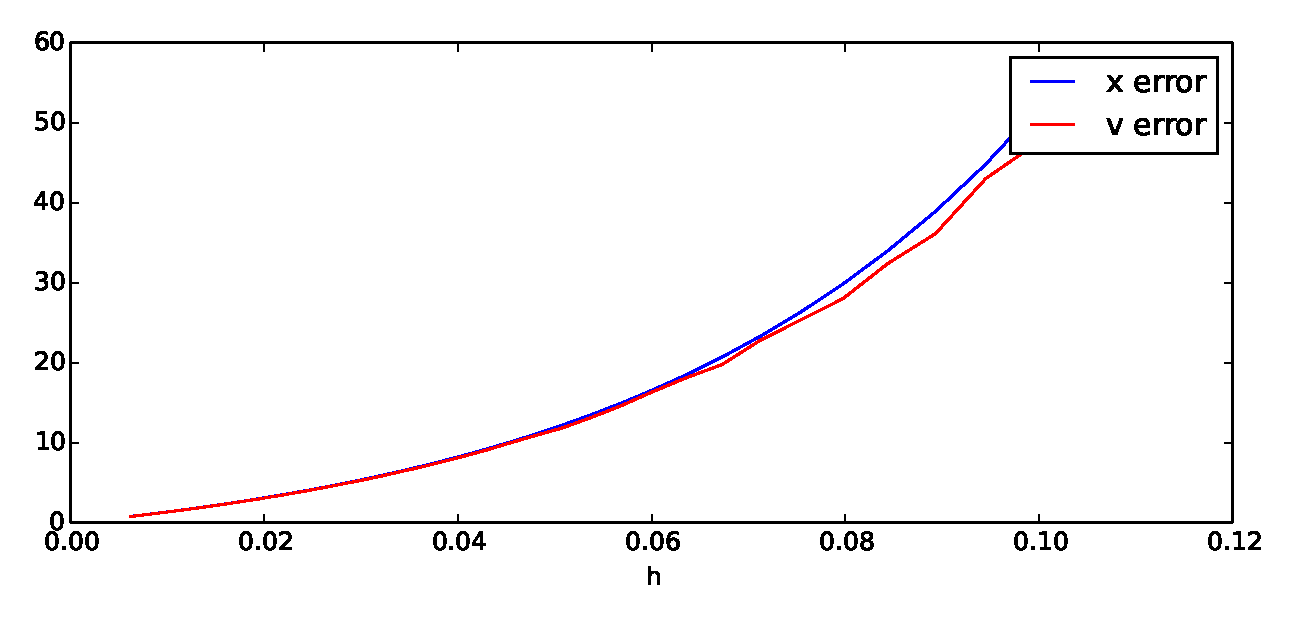
\includegraphics[width=\textwidth]{bigh.eps}
\caption{\label{fig:bigh}Truncation error vs. $h$ for large values of
$h$.}
\end{figure}

\begin{figure}
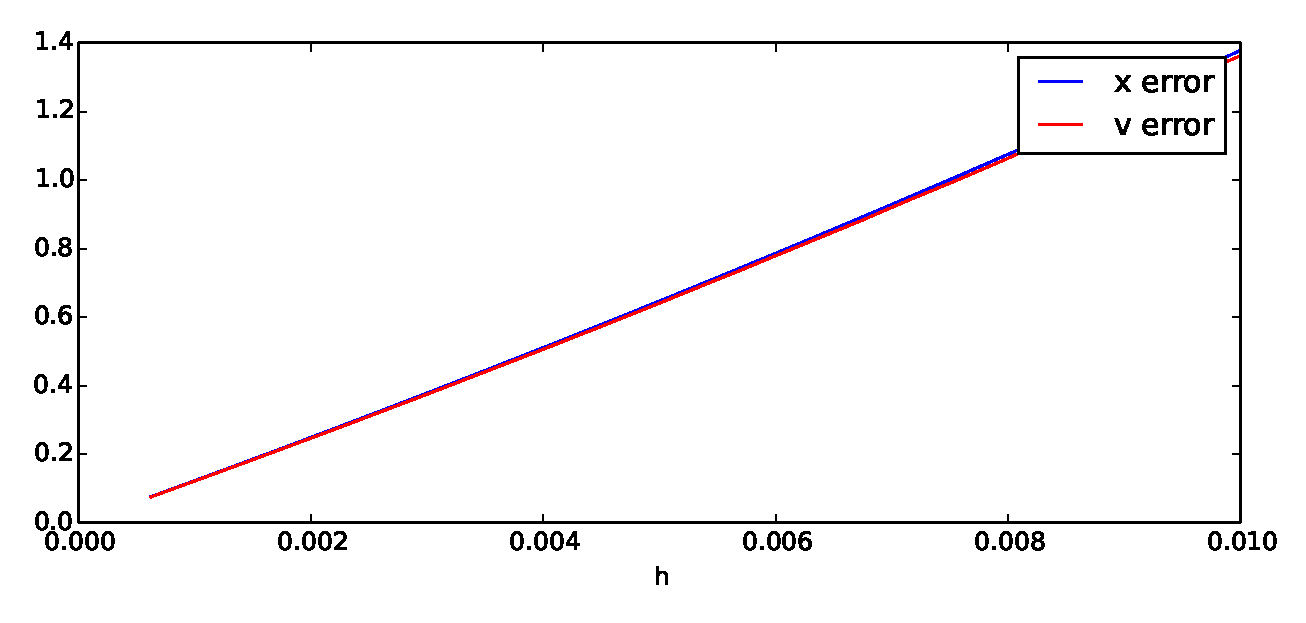
\includegraphics[width=\textwidth]{smallh.eps}
\caption{\label{fig:smallh}Truncation error vs. $h$ for small values of
$h$.}
\end{figure}

\section{Energy conservation in explicit Euler method}

Given $E=x^2+v^2$, we can plot energy as a function of time with our
numerical solutions for $x$ and $v$. Figure \ref{fig:explicit_E} shows
that the numerical solution does not exhibit energy conservation, instead
showing energy increasing over time.

\begin{figure}
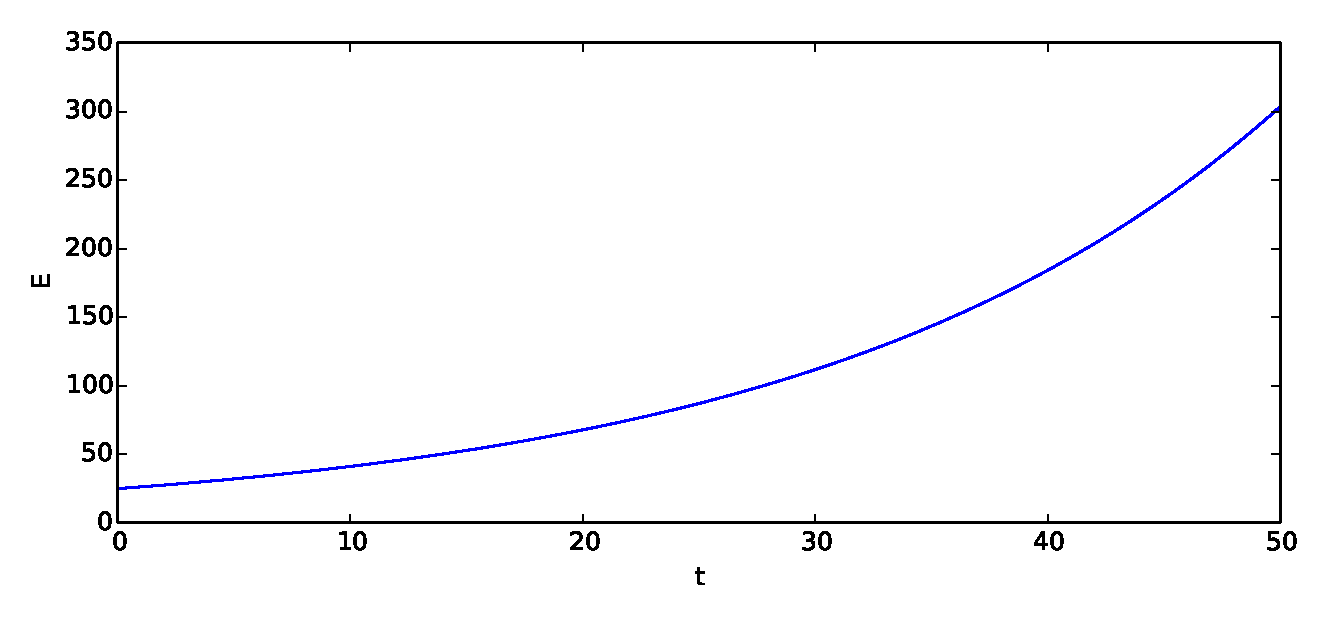
\includegraphics[width=\textwidth]{explicit_E.eps}
\caption{\label{fig:explicit_E}$E(t)$ as determined from explicit-Euler-method numerical
solutions to $x(t)$ and $v(t)$.}
\end{figure}

\begin{figure}
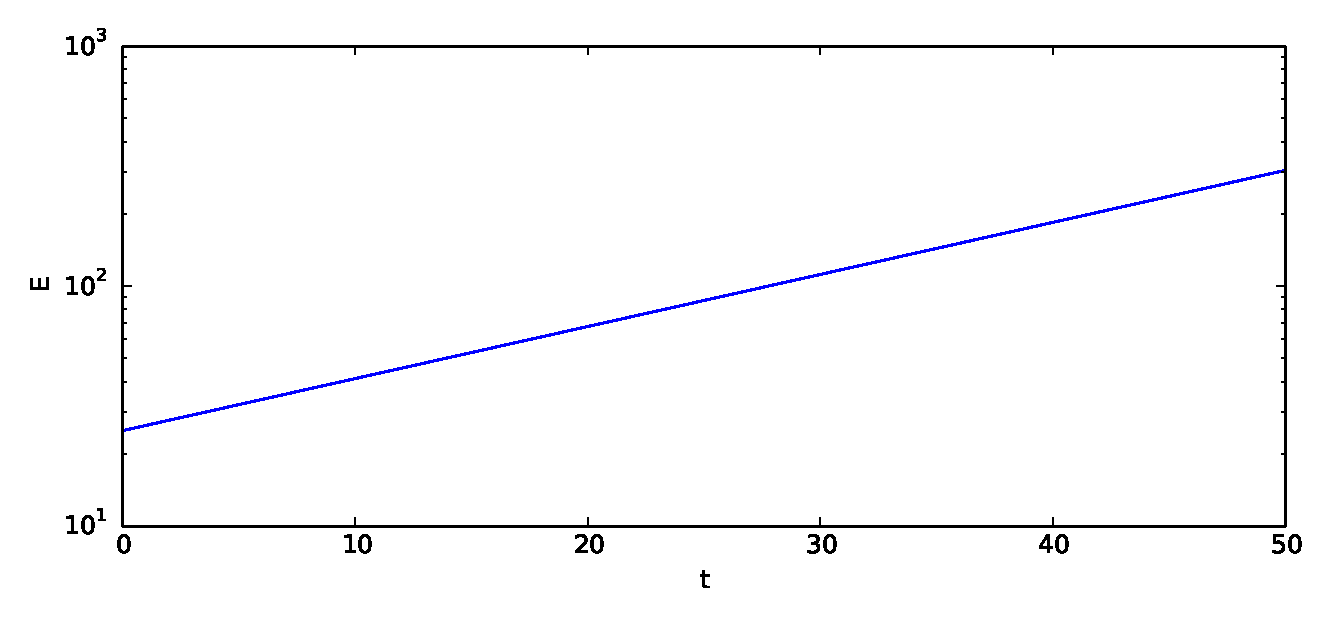
\includegraphics[width=\textwidth]{explicit_E_log.eps}
\caption{\label{fig:explicit_E_log}$E(t)$ as determined from explicit-Euler-method numerical
solutions, with $E$ plotted on a log scale. The linear graph shows that $E(t)$ increases
exponentially with $t$.}
\end{figure}

Visually, the trend appears to be quadratic or exponential. By generating
a log plot in figure \ref{fig:explicit_E_log}, we confirm that growth trend of $E(t)$ is
indeed exponential.

\section{Implicit Euler method}

The implicit Euler method uses values at $t+h$ to updates values at $t+h$, as
opposed to the explicit Euler method which used values at $t$ to updates values
at $t+h$.
\begin{align*}
x_{i+1} &= x_i + hv_{i+1}. \\
v_{i+1} &= v_i - hx_{i+1}.
\end{align*}

We obtain $x(t+h)$ and $v(t+h)$ in terms of $x(t)$ and $v(t)$ with some algebraic
manipulation. As demonstrated, the two above equations are equivalent to the
linear system:
\begin{align*}
\left(\begin{array}{cc}
1 & -h \\
h & 1
\end{array}\right)
\left(\begin{array}{c}
x_{i+1} \\
v_{i+1}
\end{array}\right)
&=
\left(\begin{array}{c}
x_i \\
v_i
\end{array}\right)
\end{align*}
Using \emph{Mathematica}, we find that:
\begin{align*}
x_{i+1} &= \frac{x_i + hv_i}{h^2 + 1}. \\
v_{i+1} &= \frac{v_i - hx_i}{h^2 + 1}.
\end{align*}
Using this method and the same conditions as in figure \ref{fig:explicit}, we can
generate new numerical solutions for $x$ and $v$ in figure \ref{fig:implicit}.
We also show the global error between the implicit and analytic solutions
in figure \ref{fig:implicit_error}.

With the new numerical solutions, we also generate a new solution for
$E(t)$, plotted in figure \ref{fig:implicit_E}. 

\begin{figure}
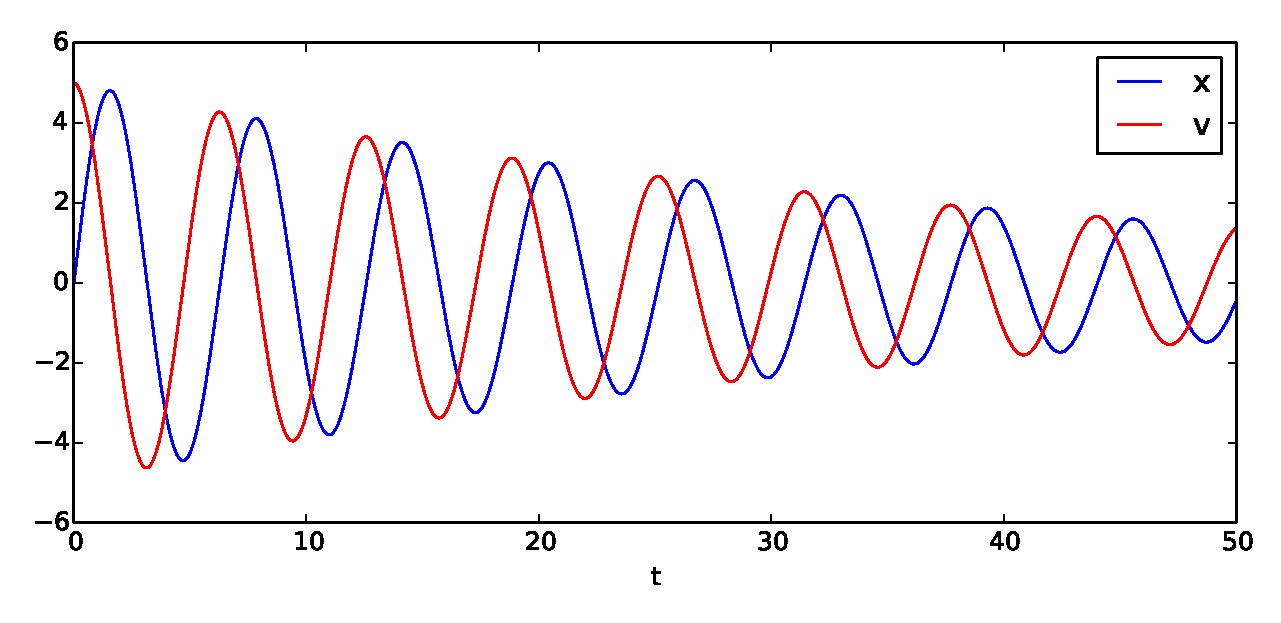
\includegraphics[width=\textwidth]{implicit.eps}
\caption{\label{fig:implicit}Numerical solutions for $x(t)$ and $v(t)$ as calculated by
the implicit Euler method.}
\end{figure}

\begin{figure}
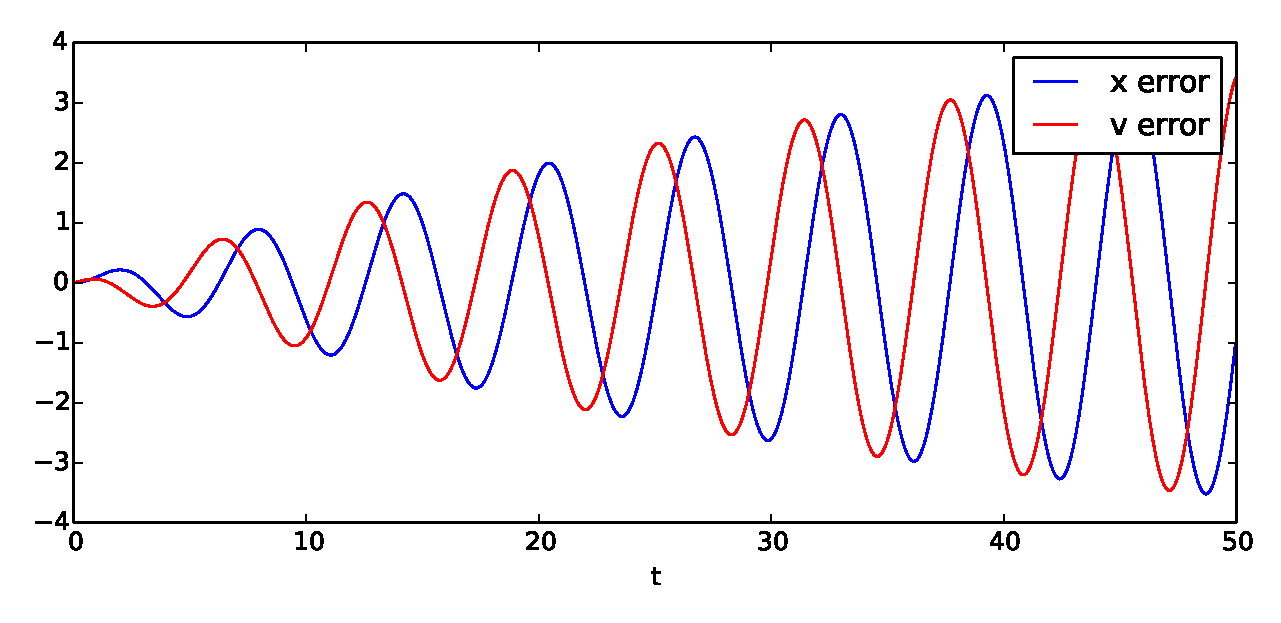
\includegraphics[width=\textwidth]{implicit_error.eps}
\caption{\label{fig:implicit_error}Truncation error for
the implicit Euler method.}
\end{figure}

\begin{figure}
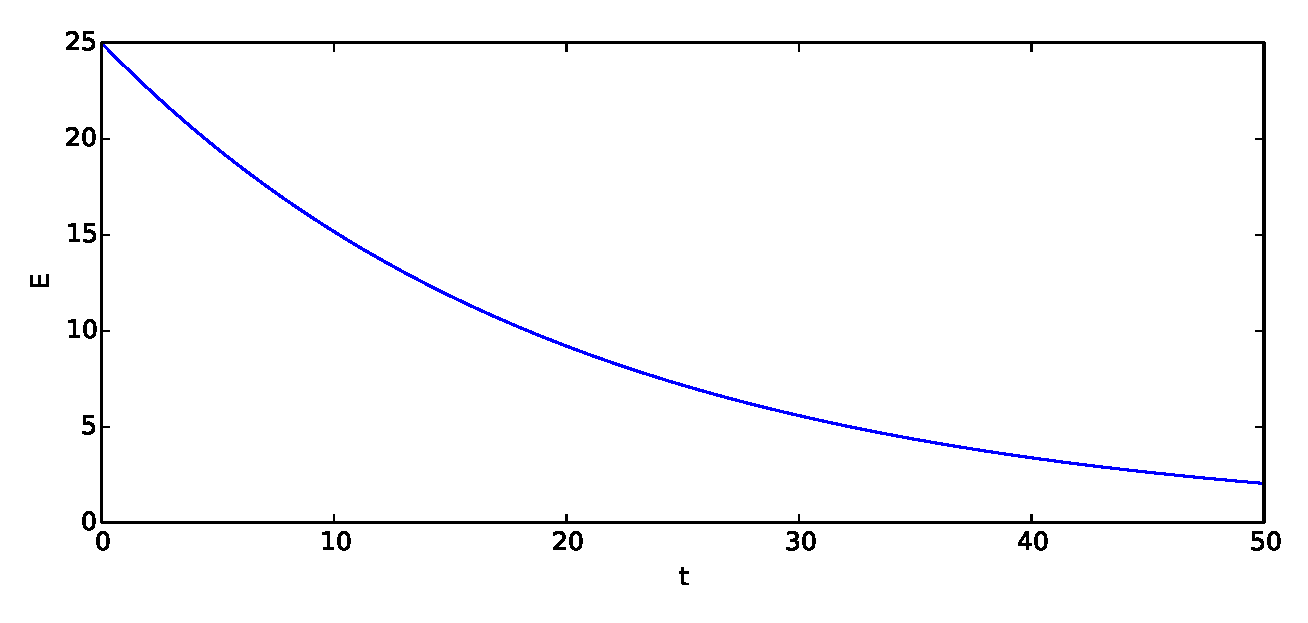
\includegraphics[width=\textwidth]{implicit_E.eps}
\caption{\label{fig:implicit_E}$E(t)$ as determined from implicit-Euler-method numerical
solutions to $x(t)$ and $v(t)$.}
\end{figure}

\section{Phase-space geometry and the non-symplectic Euler methods}

Since $E=x^2 + v^2$, and energy should be conserved in an ideal spring,
plotting the spring's trajectory in the $xv$-plane should yield a circle of radius
$\sqrt{E}$. Of course, we have already seen that the explicit and implicit Euler
methods do not conserve energy, so their phase-space trajectories will be spirals
rather than closed circles, as shows in figure \ref{fig:Euler_xv}.
These plots are generated with the same conditions as before:
$x_0 = 0, v_0 = 5, h = 0.05, s = 50$.

\begin{figure}\centering
\begin{subfigure}{0.48\textwidth}
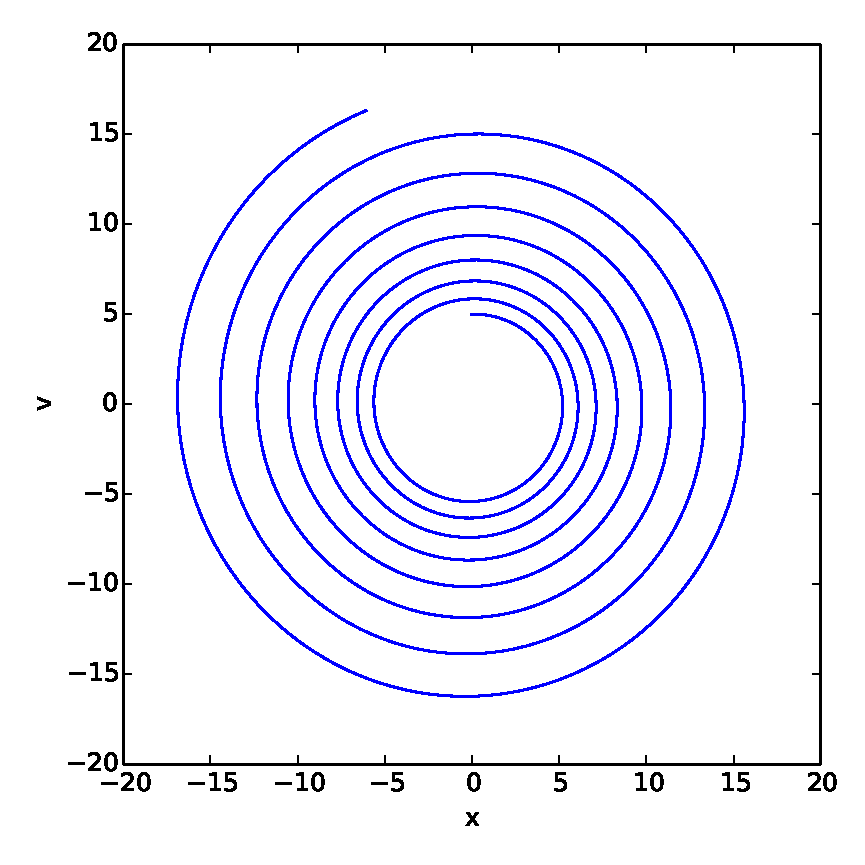
\includegraphics[width=\textwidth]{explicit_xv.eps}
\caption{explicit Euler method}
\end{subfigure}
\begin{subfigure}{0.48\textwidth}
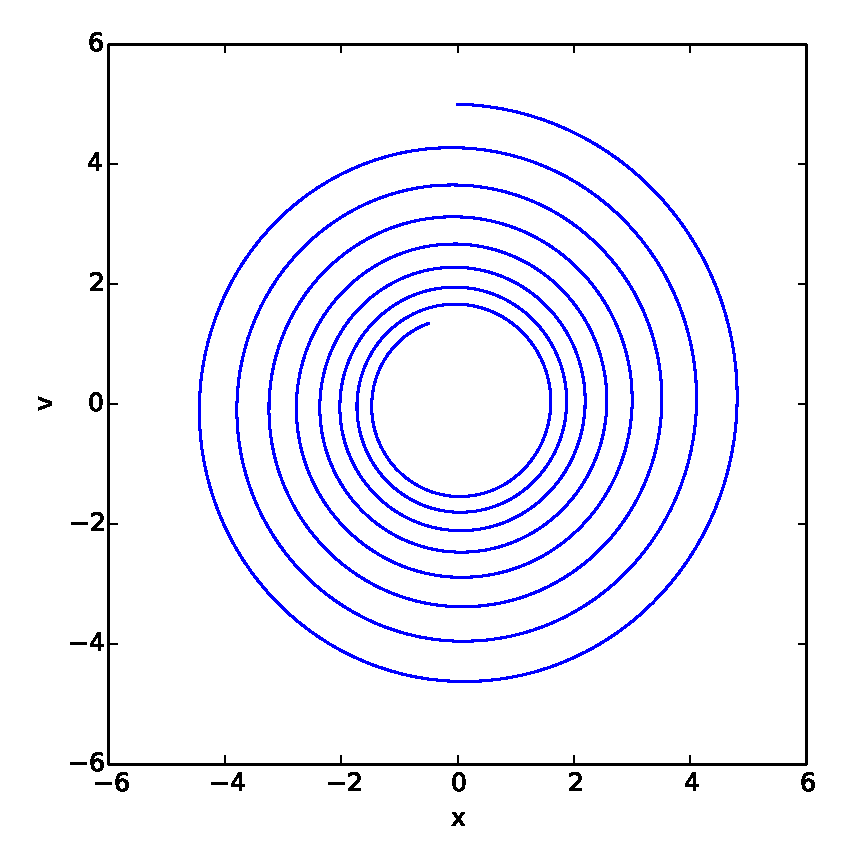
\includegraphics[width=\textwidth]{implicit_xv.eps}
\caption{implicit Euler method}
\end{subfigure}
\caption{\label{fig:Euler_xv}Phase-space trajectories for explicit and implicit
Euler methods.}
\end{figure}

\section{Implementation of symplectic Euler method}

To design a numerical method that conserves area in phase space (and thus conserves
energy), we combine the
explicit and implicit Euler methods:
\begin{align*}
x_{i+1} &= x_i + hv_i. \\
v_{i+1} &= v_i - hx_{i+1} \\
&= v_i - h(x_i + hv_i) \\
&= v_i - hx_i -h^2v_i.
\end{align*}

Figure \ref{fig:symplectic} shows the numerical solutions for $x(t)$ and $v(t)$ obtained
through this method. We immediately notice that, as expected from the analytic solution
to a spring's motion, the amplitude does not change over time in our time frame ($t=0$
to $t=50$).

Figure \ref{fig:symplectic_xv} shows the phase-space trajectory, which appears closed
in our time frame. There is a visible offset from the perfect circle traced out
by the analytic solution: sometimes the symplectic curve is inside the analytic curve,
and other times it is outside. Since the radius of the
curve is $\sqrt{E}$, this means we should expect the symplectic Euler method to yield
small oscillations in $E$. This is exactly what happens: see section 8.

\begin{figure}
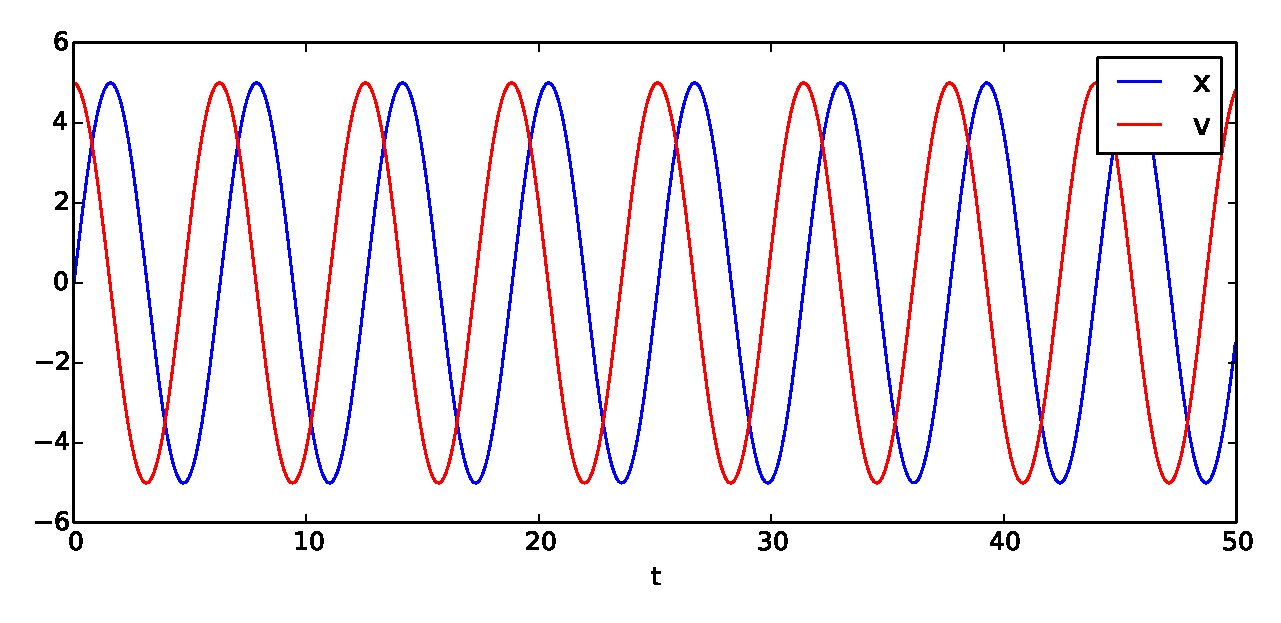
\includegraphics[width=\textwidth]{symplectic.eps}
\caption{\label{fig:symplectic} Numerical solutions for $x(t)$ and $v(t)$ as calculated
by the symplectic Euler method.}
\end{figure}

\begin{figure}
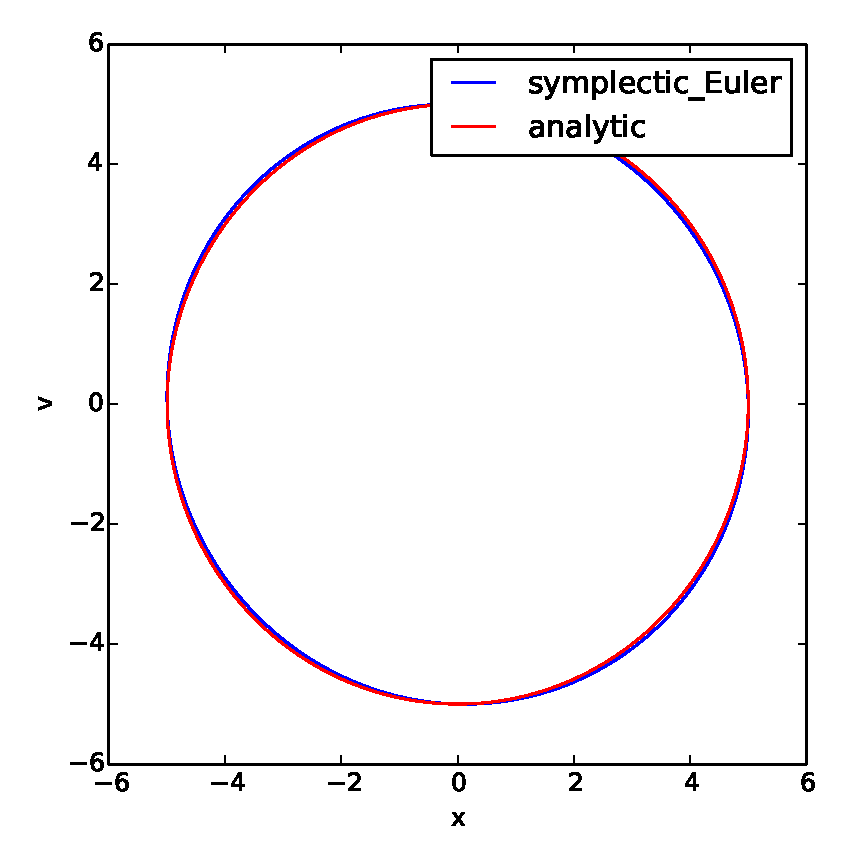
\includegraphics[width=\textwidth]{combined_xv.eps}
\caption{\label{fig:symplectic_xv} Phase-space trajectory for symplectic Euler
and analytic methods.}
\end{figure}

\section{Energy evolution of symplectic Euler method}

Though the phase-space trajectory (figure \ref{fig:symplectic_xv}) suggests that energy
is conserved with the symplectic Euler method, the calculated energy undergoes small
oscillations around the expected constant value of 25.0 (see figure \ref{fig:symplectic_E}).

\begin{figure}
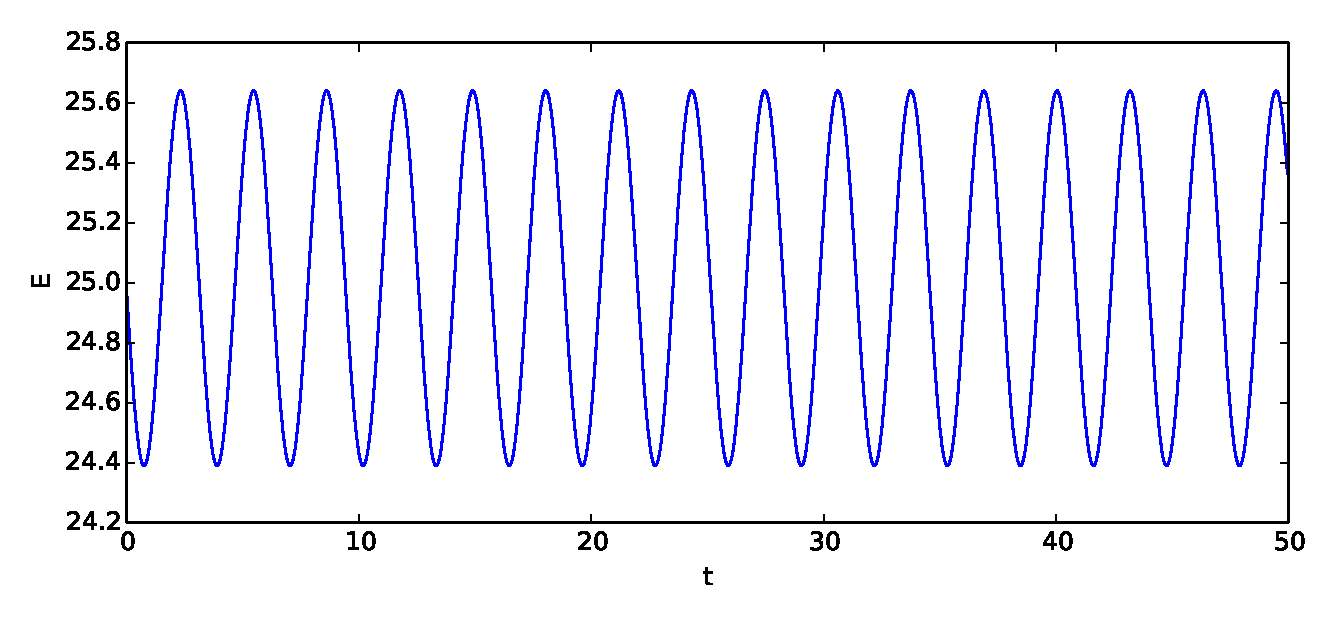
\includegraphics[width=\textwidth]{symplectic_E.eps}
\caption{\label{fig:symplectic_E} $E(t)$ for symplectic Euler method.} 
\end{figure}

\section{Long-term error in symplectic Euler method}

In addition to the small oscillations in energy, the symplectic Euler method exhibits another
imperfection: the calculated solutions for $x(t)$ and $v(t)$ lag behind the analytic solutions.
Figure \ref{fig:symplectic_error} shows this phenomenon. Note that the figure is plotted from
$t=4950$ to $t=5000$; the error is not appreciable at small times.

\begin{figure}[h!]
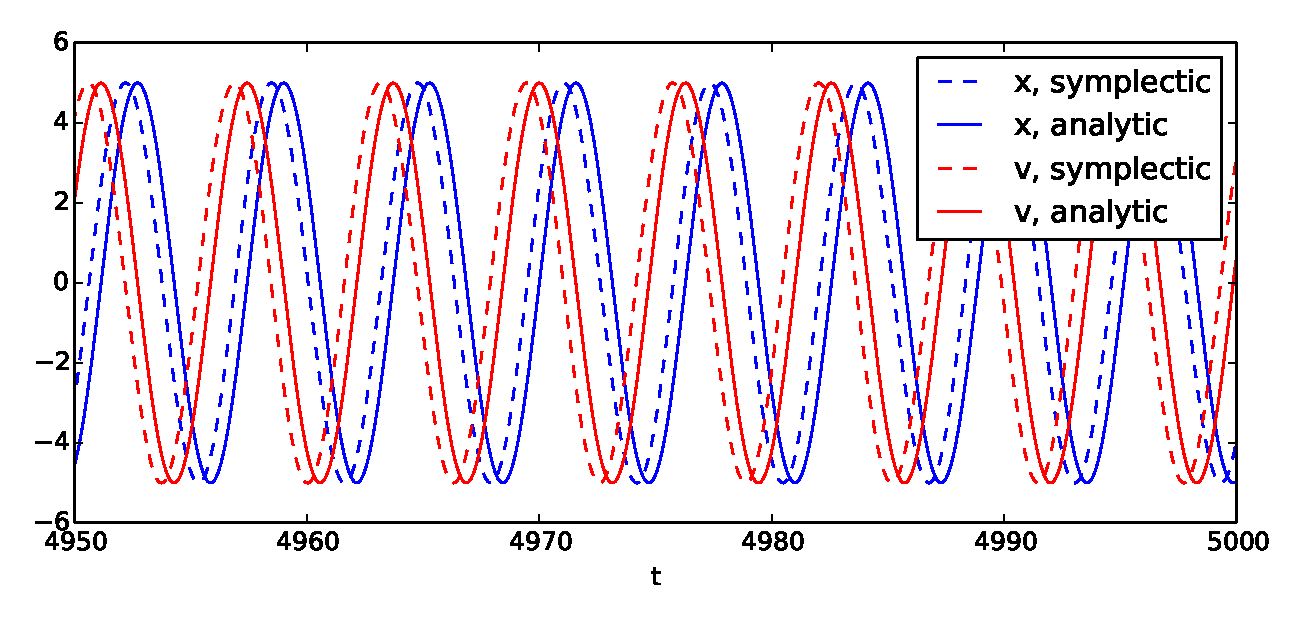
\includegraphics[width=\textwidth]{symplectic_error.eps}
\caption{\label{fig:symplectic_error} Comparison of numerical and analytic solutions for $x(t)$ and $v(t)$, showing
that at large $t$, the symplectic solution exhibits a noticeable lag.} 
\end{figure}

\end{document}
